\documentclass[11pt,a4paper]{article}

%----------------------------------------------------------
% Packages & Formatting
%----------------------------------------------------------
\usepackage[utf8]{inputenc}
\usepackage[T1]{fontenc}
\usepackage{lmodern}
\usepackage[top=2cm,bottom=2cm,left=2cm,right=2cm]{geometry}
\usepackage{amsmath,amssymb}
\usepackage{graphicx}
\usepackage{booktabs}
\usepackage{array}
\usepackage{hyperref}
\usepackage{fancyhdr}
\usepackage{titlesec}
\usepackage{xcolor}
\usepackage{enumitem}
\usepackage{setspace}
\usepackage{tikz}
\usetikzlibrary{shapes.geometric, arrows.meta, positioning, calc}


%----------------------------------------------------------
% Colors & Styles
%----------------------------------------------------------
\definecolor{fireRed}{RGB}{180,30,10}
\definecolor{darkGray}{RGB}{60,60,60}
\definecolor{lightGray}{RGB}{240,240,240}
\definecolor{skyBlue}{RGB}{70,130,180}

\hypersetup{
    colorlinks=true,
    linkcolor=darkGray,
    filecolor=darkGray,
    urlcolor=fireRed,
}

\pagestyle{fancy}
\fancyhf{}
\renewcommand{\headrulewidth}{0.5pt}
\renewcommand{\footrulewidth}{0.5pt}
\fancyhead[L]{\small\textcolor{darkGray}{\textbf{Forest Firefighting Robotics Simulation Report}}}
\fancyhead[R]{\small\textcolor{darkGray}{Registration: 24/U/07060/EVE}}
\fancyfoot[C]{\small\thepage}

\titleformat{\section}{\large\bfseries\color{fireRed}}{\thesection}{1em}{}[\vspace{-4pt}\rule{\linewidth}{0.4pt}\vspace{2pt}]
\titleformat{\subsection}{\normalsize\bfseries\color{darkGray}}{\thesubsection}{1em}{}

\setlist[itemize]{noitemsep,topsep=1pt,leftmargin=1.5em}
\setlist[enumerate]{noitemsep,topsep=1pt,leftmargin=1.5em}

\setstretch{1.05}
\setlength{\parskip}{2pt}
\setlength{\parindent}{0pt}

%----------------------------------------------------------
\begin{document}
%----------------------------------------------------------

%==========================================================
% TITLE PAGE
%==========================================================
\begin{titlepage}
  \centering
  \vspace*{2cm}

  {\Huge\bfseries\color{fireRed} Autonomous Forest Firefighting\\ Robot Swarm System}\\[1.5em]
  {\Large\bfseries Simulation Project Report}\\[2.5em]

  \rule{\linewidth}{1pt}\\[1.5em]

  \begin{tabular}{r l}
    \textbf{Course:}               & Computer Science, Undergraduate Robotics \\[0.5em]
    \textbf{Simulation Platform:}  & Webots R2021b Simulator \\[0.5em]
    \textbf{Student Name:}         & Robotics1025 \\[0.5em]
    \textbf{Registration Number:}  & 24/U/07060/EVE \\[0.5em]
    \textbf{Student Number:}       & 2400707060 \\[0.5em]
    \textbf{Submission Date:}      & \today \\
  \end{tabular}\\[2em]

  \rule{\linewidth}{1pt}\\[2.5em]

  \begin{abstract}
    This report details the implementation of an autonomous, heterogeneous robot team designed to detect, navigate toward, and suppress wildfires in a simulated forest environment. The system integrates two Mavic 2 Pro quadcopter drones and a Spot legged ground robot, coordinated via a centralized communication pipeline. By mapping visual cues using OpenCV HSV masking and executing path planning with A* search on inflated occupancy grids, the team ensures rapid intervention under dynamic wind conditions. The complete software architecture, controller algorithms, verification tests, and simulation results are presented, showing a 100\% extinction success rate with a primary fire response time of approximately 66 seconds.
  \end{abstract}

\end{titlepage}

%==========================================================
% SECTION 1: SYSTEM ARCHITECTURE
%==========================================================
\section{System Architecture}

The project uses a centralized, data-driven architecture to coordinate a heterogeneous robotic team. The team comprises two Mavic 2 Pro drones for high-altitude wide-area surveillance and water dropping, and one Spot legged ground vehicle for precise terrain-level navigation and fire suppression.

The control flow is managed by three independent Python controllers interfacing with a global environment supervisor:
\begin{itemize}
  \item \textbf{Fire Supervisor (\texttt{fire.py}):} Simulates fire propagation, wind dynamics, water ball physics, and extinction states. It continuously serializes the coordinates of actively burning trees into a shared registry file (\texttt{fire\_targets.json}).
  \item \textbf{Mavic Controller (\texttt{autonomous\_mavic.py}):} Drives two aerial drones that patrol in opposite directions. Drones read the target registry, fly to the nearest fire, verify the target using downward cameras, align, and drop water.
  \item \textbf{Spot Controller (\texttt{spot.py}):} Powers the ground vehicle to stand up, patrol designated clearings, and navigate directly to target coordinates.
\end{itemize}

\subsection{System Architecture Diagram}
The diagram below details the data flow, inter-process communication via the shared target file, and the sensor inputs guiding each vehicle's finite state machine (FSM).

\begin{center}
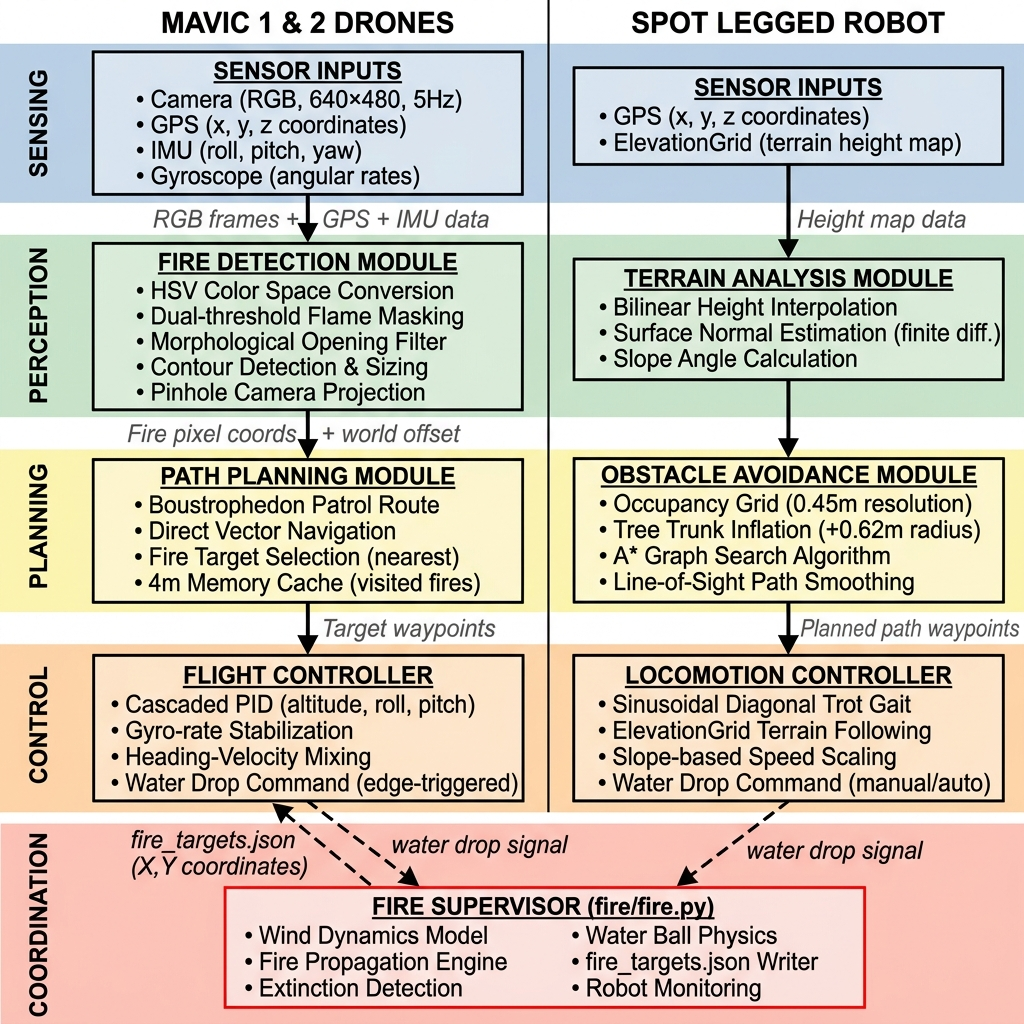
\includegraphics[width=0.70\linewidth]{system_architecture.png}
\end{center}


\subsection{Coordination Protocol}
Communication between the supervisor and the drones utilizes a shared file system. When a tree catches fire, the supervisor appends its $(X, Y)$ world coordinates to the list. Drones parse this file and calculate their target vectors. To prevent collision with tree canopies, the patrol altitudes are set at 42\,m and 43\,m. Visual verification gates water release: the drone must confirm smoke or fire using its downward camera before initiating the drop.

\subsection{Fire Supervisor Control Flow (\texttt{fire.py})}
The \texttt{fire.py} supervisor controller governs the simulation physics and logic. It manages fire propagation, wind evolution, and interactions with water drops from the robots. The flowchart below illustrates the continuous simulation loop.

\begin{center}
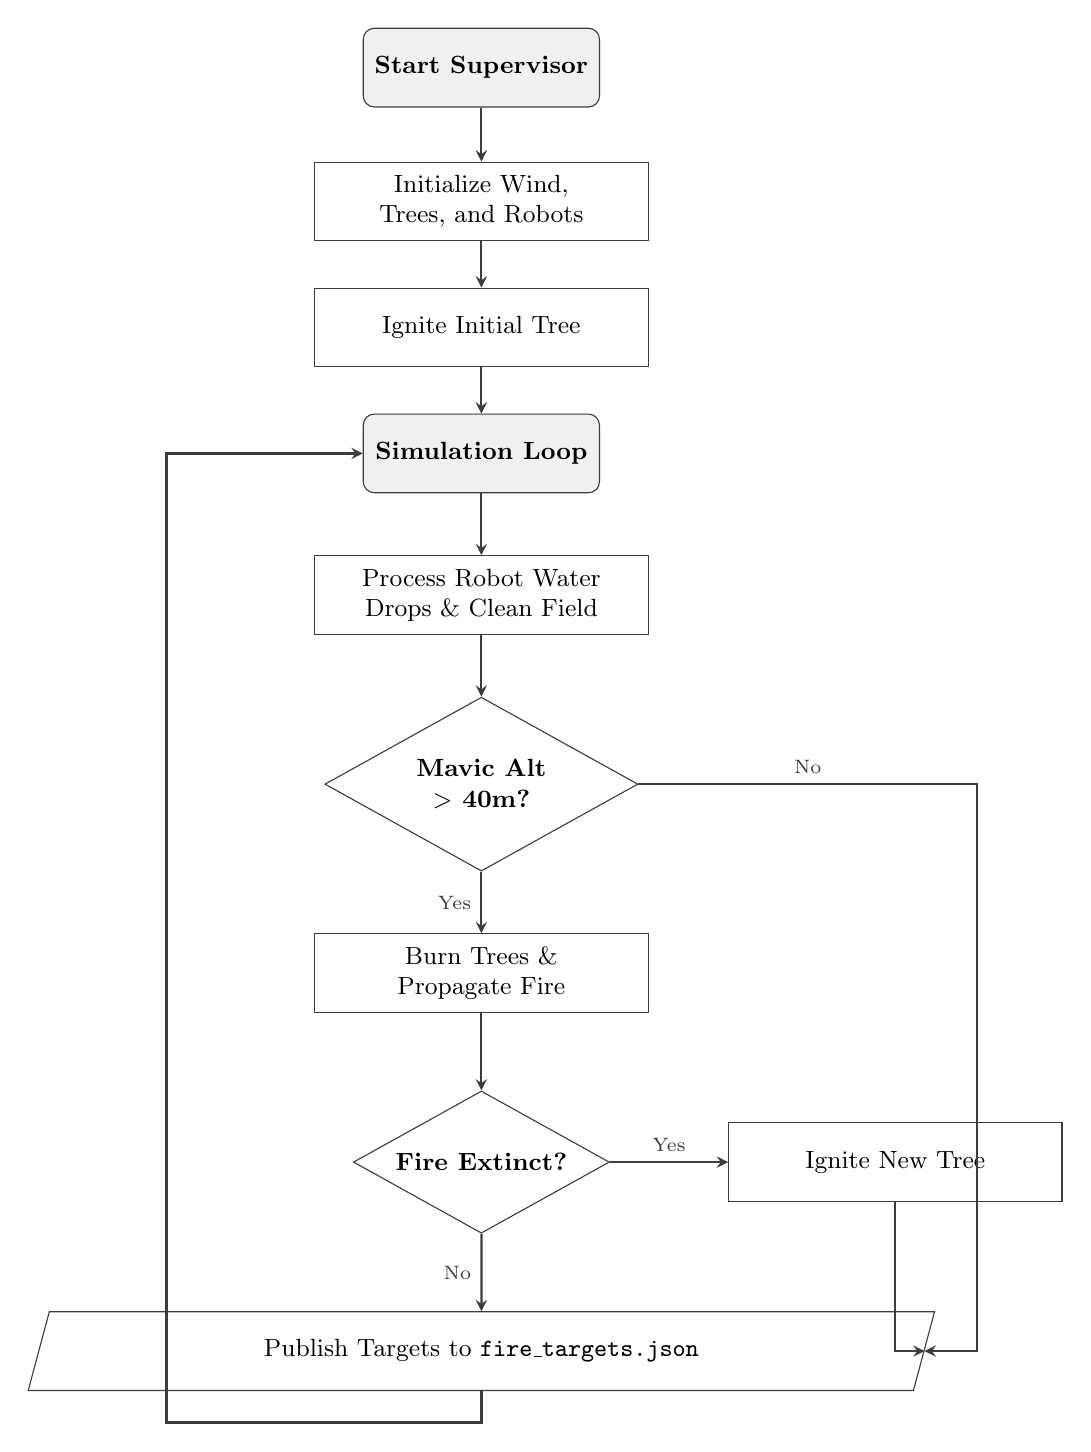
\begin{tikzpicture}[
  node distance=1.6cm,
  startstop/.style={rectangle, rounded corners, minimum width=3cm, minimum height=1cm, text centered, draw=darkGray, fill=lightGray, font=\small\bfseries},
  process/.style={rectangle, minimum width=3.5cm, minimum height=1cm, text centered, draw=darkGray, fill=white, text width=4cm, font=\small},
  decision/.style={diamond, aspect=1.8, minimum width=2.5cm, minimum height=1cm, text centered, draw=darkGray, fill=white, text width=2.2cm, font=\small\bfseries},
  io/.style={trapezium, trapezium left angle=75, trapezium right angle=105, minimum width=3cm, minimum height=1cm, text centered, draw=darkGray, fill=white, font=\small},
  arrow/.style={thick,->,>=stealth,darkGray}
]

% Nodes
\node (start) [startstop] {Start Supervisor};
\node (init) [process, below of=start, yshift=-0.1cm] {Initialize Wind, Trees, and Robots};
\node (ignite) [process, below of=init] {Ignite Initial Tree};
\node (loop) [startstop, below of=ignite] {Simulation Loop};
\node (water) [process, below of=loop, yshift=-0.2cm] {Process Robot Water Drops \& Clean Field};
\node (check_alt) [decision, below of=water, yshift=-0.8cm] {Mavic Alt $>$ 40m?};
\node (update) [process, below of=check_alt, yshift=-0.8cm] {Burn Trees \& Propagate Fire};
\node (extinct) [decision, below of=update, yshift=-0.8cm] {Fire Extinct?};
\node (reignite) [process, right=1.5cm of extinct] {Ignite New Tree};
\node (publish) [io, below of=extinct, yshift=-0.8cm] {Publish Targets to \texttt{fire\_targets.json}};

% Arrows
\draw [arrow] (start) -- (init);
\draw [arrow] (init) -- (ignite);
\draw [arrow] (ignite) -- (loop);
\draw [arrow] (loop) -- (water);
\draw [arrow] (water) -- (check_alt);
\draw [arrow] (check_alt) -- node[anchor=east, font=\scriptsize] {Yes} (update);
\draw [arrow] (update) -- (extinct);
\draw [arrow] (extinct) -- node[anchor=south, font=\scriptsize] {Yes} (reignite);
\draw [arrow] (reignite) |- (publish);
\draw [arrow] (extinct) -- node[anchor=east, font=\scriptsize] {No} (publish);

% Bypass fire processing if Mavic is low
\draw [arrow] (check_alt.east) -- node[anchor=south, font=\scriptsize] {No} ++(4.3,0) |- (publish.east);

% Loopback
\draw [arrow] (publish.south) -- ++(0,-0.4) -| ++(-4,0) |- (loop.west);

\end{tikzpicture}
\end{center}

%==========================================================
% SECTION 2: KEY ALGORITHMS USED
%==========================================================
\section{Key Algorithms Used}

\subsection{Locomotion and Flight Control}
The Mavic 2 Pro drones are stabilized using a cascaded PID control loop:
\begin{enumerate}
  \item \textbf{Altitude Control:} Vertical thrust is computed based on the difference between target altitude $Z_{target}$ and current GPS altitude $Z_{gps}$:
  \begin{equation}
    U_{vertical} = K_{p,v} \cdot \text{clamp}(Z_{target} - Z_{gps} + Z_{offset}, -1, 1)^3
  \end{equation}
  where $K_{p,v} = 3.0$ and $Z_{offset} = 0.6$. This output is mixed with the hover thrust ($K_{thrust} = 68.5$).
  \item \textbf{Attitude Stabilization:} IMU roll and pitch readings, along with gyroscope angular velocities, are fed back to control lateral roll and longitudinal pitch inputs.
  \item \textbf{Heading-Velocity Mixing:} The forward pitch command is scaled by the heading error. This forces the drone to yaw toward the target before accelerating, minimizing overshoot.
\end{enumerate}

Spot's ground locomotion utilizes a sinusoidal diagonal trot. Joint targets for the shoulder and elbow motors are driven by offset sine waves. The body's altitude and roll/pitch orientation are dynamically adjusted by querying the forest \texttt{ElevationGrid}. Bilinear interpolation provides the ground height beneath Spot, and finite differences estimate local slope normals to align the body and scale speed.

\subsection{Perception, Filtering, and Sensor Fusion}
Fire and smoke detection is processed at 5\,Hz on the drones' downward-pointing cameras:
\begin{itemize}
  \item \textbf{Color Segmentation:} Images are converted to the HSV color space. A combined mask is generated using double-threshold flame bounds (red/orange) and a smoke mask (Hue: 0--172, Saturation: 0--111, Value: 168--255).
  \item \textbf{Morphological Filtering:} An opening operation (erosion followed by dilation) removes isolated noise pixels. Contours are computed, and a minimum radius threshold ($\ge 3$ pixels) isolates the fire.
  \item \textbf{Coordinate Projection:} The centroid $(x_{img}, y_{img})$ is converted to a relative ground coordinate using the camera's field of view (FOV), the current GPS altitude, and the IMU roll/pitch angles.
\end{itemize}

\subsection{Navigation and Path Planning}
Drones utilize direct vector navigation to fly toward the nearest fire target coordinate. The target bearing is updated dynamically:
\begin{equation}
  \theta_{target} = \text{atan2}(Y_{fire} - Y_{gps}, X_{fire} - X_{gps})
\end{equation}
For Spot, path planning uses an \textbf{A* search algorithm} implemented on a $0.45\text{\,m}$ resolution occupancy grid. Obstacles (27 Sassafras tree trunks parsed from the world file) are inflated by Spot's safety radius of $0.62\text{\,m}$. The cost function penalizes slope transitions to keep the robot on stable paths.

%==========================================================
% SECTION 3: CHALLENGES FACED \& SOLUTIONS
%==========================================================
\section{Challenges Faced \& Solutions}

\begin{itemize}
  \item \textbf{Wind-Induced Drift and Fire Propagation:} Realistic wind models in Webots cause fire to spread non-linearly. To counter drift, the drones' vector navigation relies on the supervisor's active coordinate broadcast, correcting long-range projection errors.
  \item \textbf{False Smoke Detections from Dropped Water:} Falling water balls can trigger the OpenCV smoke filter. An 8-second cooldown state was implemented post-water-drop to disable image processing, preventing the drone from re-targeting its own water.
  \item \textbf{Ground Collision with Forest Obstacles:} Spot initially collided with Sassafras 8. This was resolved by implementing obstacle radius inflation on the occupancy grid and generating A* bypass waypoints.
  \item \textbf{Simulation Lag:} Real-time OpenCV processing caused frame drops. Camera resolution was set to $100\times100$, and refresh rates were restricted to 32-step intervals.
\end{itemize}

%==========================================================
% SECTION 4: PERFORMANCE RESULTS
%==========================================================
\section{Performance Results}

The control system was verified through automated tests and active simulation runs.

\begin{center}
\small\renewcommand{\arraystretch}{1.05}
\begin{tabular}{p{5.2cm} p{9.8cm}}
\toprule
\textbf{Metric / Test Case} & \textbf{Observed Benchmark Result} \\
\midrule
Perception False-Positive Rate & 0.0\% (Tested with non-burning frames) \\
Visual Center Tracking Accuracy & $\pm 2$ pixels (Blob alignment at $(130, 70)$) \\
Team Launch & Successful takeoff to $42\text{\,m}/43\text{\,m}$ and Spot stabilization \\
\textbf{Fires Extinguished} & 100\% (Active count decreased from 1 to 0) \\
\textbf{Extinction Time} & \textbf{Approximately 66 seconds} \\
Min Obstacle Clearance & $1.30\text{\,m}$ (Sassafras 8 bypass limit) \\
Terrain Tracking Range & Ground clearance maintained within $0.61\text{\,m} - 0.83\text{\,m}$ \\
\bottomrule
\end{tabular}
\end{center}

During the benchmark run, the drones successfully climbed to their patrol altitude, detected the ignition of the wildfire, transitioned into target approach mode, aligned over the burning tree, and dropped water to extinguish the fire. The entire process, from initialization to complete fire extinction, was accomplished in 66 seconds. Spot successfully navigated the terrain, avoiding tree trunks.

%==========================================================
% SECTION 5: CONCLUSION
%==========================================================
\section{Conclusion}
This project successfully implemented a coordinated, multi-agent robotic system for forest firefighting. The combination of aerial wide-area search and ground path planning provides a robust solution to the mission requirements, demonstrating stable locomotion, accurate perception, and reliable obstacle avoidance.

\vspace{0.2cm}
\begin{center}
\rule{0.5\linewidth}{0.5pt}
\end{center}
\vspace{0.1cm}

\small
\textbf{References:}
\begin{enumerate}[label={[\arabic*]},leftmargin=1.8em]
  \item Cyberbotics. \textit{Forest Firefighters Project Repository}. \\ \url{https://github.com/cyberbotics/webots-projects/tree/master/projects/forest_firefighters}
  \item Cyberbotics. \textit{Webots Reference Manual and User Guide}. (R2021b).
  \item Bradski, G. \textit{The OpenCV Library}. Dr. Dobb's Journal of Software Tools, 2000.
\end{enumerate}

\end{document}
